%!TEX root =  ../Report.tex
% %Here are some subsections so that they will appear on the contents
\subsection{Classifiers}

%Classification on the combined set of features was conducted against three classifier models, Random Forest (RF), XGBoost and K-Nearest Neighbour (KNN).

\subsubsection{Random Forest (RF)}
\label{sec:RF}

Basically existing research doesn't have any models or research using a random forest ensemble classifier, only decision trees in \parencite{9360747}

\begin{table}[h]
\centering
\caption{Parameters for Random Forest Classifier}
\label{tab:rf-params}
\begin{tabular}{|l|l|l|l|}
\hline
\textbf{Parameter} & \textbf{Description} & \textbf{Value}  \\ \hline
n\_estimators & The number of trees in the forest & 100\\
criterion & Function to measure the quality of a split. & gini\\
max\_depth & Maximum depth of the tree. &  None \\
min\_samples\_split & Minimum samples required to split an internal node. & 2 \\ 
min\_samples\_leaf & Minimum samples required to be at a leaf node. & 1 \\
max\_features & Maximum features to consider when splitting.  & auto \\
bootstrap & To bootstrap samples when constructing trees & True \\
class\_weight & Weights associated with classes & None  \\
random\_state & The random seed & 1234 \\ \hline
\end{tabular}
\end{table}

% \begin{table}[h]
% \centering
% \caption{RF Model Metrics}
% \label{tab:rf-metrics}
% \begin{tabular}{|l|l|l|l|l|l|l|}
% \hline
% \textbf{Model} & \textbf{Data Subset} & \textbf{Accuracy} & \textbf{Precision} & \textbf{Recall} & \textbf{F1} & \textbf{Time} \\ \hline
% Base & 80\% & 0.997 & 0.955 & 0.882 & 0.916 & 00:02:34:59 \\ \hline
% Base & 100\% & 0.997 & 0.997 & 0.997 & 0.997 & 00:00:30:60 \\ \hline
% \end{tabular}
% \end{table}

\begin{table}[h]
\centering
\caption{RF Model Metrics}
\label{tab:rf-metrics}
\begin{tabular}{|l|l|l|l|l|l|}
\hline
\textbf{Model} & \textbf{Data Subset} & \textbf{Accuracy} & \textbf{Precision} & \textbf{Recall} & \textbf{F1}  \\ \hline
Base & 80\% & 0.997 & 0.955 & 0.882 & 0.916  \\ \hline
Base & 100\% & 0.997 & 0.997 & 0.997 & 0.997 \\ \hline
\end{tabular}
\end{table}

\begin{table}[h]
\centering
\caption{RF Model v2}
\label{tab:rf-model2}
\begin{tabular}{|l|l|l|l|l|l|l|l|}
\hline
\textbf{Device} & \textbf{Model} & \textbf{Data Size} & \textbf{AUC} & \textbf{Precision} & \textbf{Recall} & \textbf{Accuracy} & \textbf{F1}  \\ \hline
GPU & Optimised & 100\% & 99.99 & 99.66 & 99.67 & 99.67 & 99.66 \\ \hline
\end{tabular}
\end{table}

\paragraph{Confusion Matrix}

\begin{figure}[H]
    \centering
    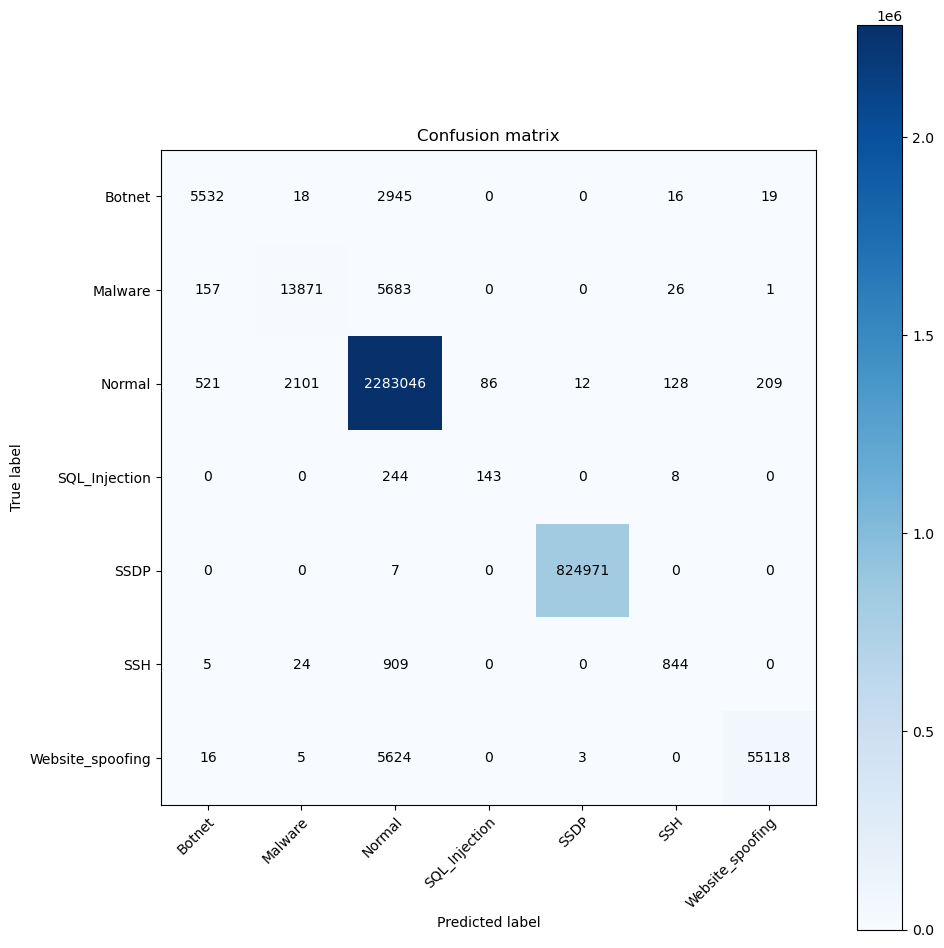
\includegraphics[width=0.85\textwidth]{Appendices/NN Confusion Matrix 3-04-23.png}
    \caption{RF Confusion Matrix}
    \label{fig:rf_confusion_matrix}
\end{figure}
